\documentclass[aspectratio=169]{beamer}
%\documentclass[aspectratio=43]{beamer}

\usepackage{graphicx}  % Required for including images
\usepackage{natbib}
\usepackage{booktabs} % Top and bottom rules for tables
\usepackage{amssymb,amsthm,amsmath}
\usepackage{exscale}
\usepackage{natbib}
\usepackage{tikz}
\usepackage{listings}
\usepackage{color}
\usepackage{animate}
\usepackage{bm}
\usepackage{etoolbox}

% Setup TikZ
\usepackage{tikz}
\usetikzlibrary{arrows}
\tikzstyle{block}=[draw opacity=0.7,line width=1.4cm]
% Setup hyperref
\usepackage{hyperref}
\hypersetup{colorlinks=true}
\hypersetup{citecolor=porange}
\hypersetup{urlcolor=porange!80!}
\hypersetup{linkcolor=porange}

\newtheorem{proposition}{Proposition}
\newtheorem{remark}{Remark}
\newtheorem{principle}{Principle}

%% Writing quarters
\newcommand{\wQ}[1]{{\textcolor{white}{Q#1}}}
\newcommand{\bQ}[1]{{Q#1}}

% Uncomment appropriate command to disable/enable hiding
%\newcommand{\mypause}{\pause}
\newcommand{\mypause}{}
\newcommand{\myb}[1]{{\color{blue} {#1}}}

%% Commonly used macros
\newcommand{\eqr}[1]{Eq.\thinspace(#1)}
\newcommand{\pfrac}[2]{\frac{\partial #1}{\partial #2}}
\newcommand{\pfracc}[2]{\frac{\partial^2 #1}{\partial #2^2}}
\newcommand{\pfraca}[1]{\frac{\partial}{\partial #1}}
\newcommand{\pfracb}[2]{\partial #1/\partial #2}
\newcommand{\pfracbb}[2]{\partial^2 #1/\partial #2^2}
\newcommand{\spfrac}[2]{{\partial_{#1}} {#2}}
\newcommand{\mvec}[1]{\mathbf{#1}}
\newcommand{\gvec}[1]{\boldsymbol{#1}}
\newcommand{\script}[1]{\mathpzc{#1}}
\newcommand{\eep}{\mvec{e}_\phi}
\newcommand{\eer}{\mvec{e}_r}
\newcommand{\eez}{\mvec{e}_z}
\newcommand{\iprod}[2]{\langle{#1}\rangle_{#2}}

\newcommand{\gcs}{\nabla_{\mvec{x}}}
\newcommand{\gvs}{\nabla_{\mvec{v}}}
\newcommand{\gps}{\nabla_{\mvec{z}}}
\newcommand{\dtv}{\thinspace d^3\mvec{v}}
\newcommand{\dtx}{\thinspace d^3\mvec{x}}


\DeclareMathAlphabet{\mathpzc}{OT1}{pzc}{m}{it}

%% Autoscaled figures
\newcommand{\incfig}{\centering\includegraphics}
\setkeys{Gin}{width=0.9\linewidth,keepaspectratio}

%Make the items smaller
\newcommand{\cramplist}{
	\setlength{\itemsep}{0in}
	\setlength{\partopsep}{0in}
	\setlength{\topsep}{0in}}
\newcommand{\cramp}{\setlength{\parskip}{.5\parskip}}
\newcommand{\zapspace}{\topsep=0pt\partopsep=0pt\itemsep=0pt\parskip=0pt}

\newcommand{\backupbegin}{
   \newcounter{finalframe}
   \setcounter{finalframe}{\value{framenumber}}
}
\newcommand{\backupend}{
   \setcounter{framenumber}{\value{finalframe}}
}

\usetheme[bullet=circle,% Use circles instead of squares for bullets.
          titleline=true,% Show a line below the frame title.
          ]{Princeton}

\title[{\tt }]{Discontinuous Galerkin Schemes, Explicit/Implicit Time-stepping}%
\author[https://ast560.rtfd.io]%
{Ammar H. Hakim ({\tt ammar@princeton.edu}) \inst{1}}%

\institute[PPPL]
{ \inst{1} Princeton Plasma Physics Laboratory, Princeton, NJ %
}

\date[4/1/2021]{Princeton University, Course AST560, Spring 2021}

\begin{document}

\begin{frame}[plain]
  \titlepage
\end{frame}

% ----------------------------------------------------------------
\begin{frame}{What are discontinuous Galerkin schemes?}

  \begin{block}{}
    Discontinuous Galerkin schemes are a class of \emph{Galerkin}
    schemes in which the solution is represented using \emph{piecewise
      discontinuous} functions.
  \end{block}
  \mypause
  \begin{itemize}
    \item \emph{Galerkin} minimization
    \item Piecewise \emph{discontinuous} representation
  \end{itemize}
  
\end{frame}  

\begin{frame}{Weak-equality and recovery}
  \begin{itemize}\cramplist
  \item It is important to remember that the discontinuous Galerkin
    solution is a \emph{representation} of the solution and not the
    solution itself.
  \item Notice that even a continuous function will, in general, have
    a discontinuous \emph{representation} in DG.
  \end{itemize}
  \mypause%
  We can formalize this idea using the concept of \emph{weak-equality}
  by stating that DG only determines the solution to an
  \emph{equivalence class of weakly-equal functions}.
  
\end{frame}

% ----------------------------------------------------------------  

\begin{frame}{Weak-equality and recovery}
  \small
  \begin{itemize}
  \item Notice that weak-equality depends on the function space as
    well as the inner-product we selected.
  \item The Galerkin $L_2$ minimization is equivalent to, for example,
    restating that
    \begin{align*}
      f'(x,t) \doteq G[f]
    \end{align*}
    This implies
    \begin{align*}
      \left(\psi_k, f'(x,t)- G[f] \right) = 0
    \end{align*}
    which is exactly what we obtained by minimizing the error defined    
    using the  $L_2$ norm. \mypause
  \item Hence, we can say that the \emph{DG scheme only determines the
      solution in the weak-sense}, that is, all functions that are
    weakly equal to DG representation can be potentially interpreted
    as the actual solution.
  \item This allows a powerful way to construct schemes with desirable
    properties by \emph{recovering} weakly-equal functions using the
    DG representations.
  \end{itemize}

\end{frame}

% ----------------------------------------------------------------  
\begin{frame}{Example of recovery: Exponential recovery in a cell}

  \begin{itemize}
  \item Consider we have a linear representation of the particle
    distribution function $f_h(x) = f_0 + x f_1$ in a cell.
  \item We can use this to \emph{reconstruct} an exponential function
    that has the desirable property that it is \emph{positive}
    everywhere in the cell. That is, we want to find
    \begin{align*}
      \exp(g_0 + g_1 x) \doteq f_0 + x f_1
    \end{align*}
  \item This will lead to a coupled set of nonlinear equations to
    determine $g_0$ and $g_1$
  \item Note that this process is not always possible: we need $f_0>0$
    as well as the condition $|f_1| \le 3 f_0$. Otherwise, the $f_h$
    is not realizable (i.e. there is no positive distribution function
    with the same moments as $f_h$).
  \end{itemize}
\end{frame}

% ----------------------------------------------------------------

\begin{frame}{Example of recovery: Exponential recovery in a cell}
  \begin{figure}
    \setkeys{Gin}{width=0.5\linewidth,keepaspectratio}
    \incfig{exp-fit-1.png}
    \incfig{exp-fit-2.png}
    \caption{Recovery of exponential function (black) from linear
      function (red). Left plot is for $f_0 = 1$, $f_1 = 1$ and right
      for $f_0 = 1$ and $f_1 = 2$.}
  \end{figure}  
\end{frame}

% ----------------------------------------------------------------

\begin{frame}{Discontinuous Galerkin scheme for linear advection}
  Consider the 1D passive advection equation on $I\in [L,R]$
  \begin{align*}
    \pfrac{f}{t} + \lambda \pfrac{f}{x} = 0
  \end{align*}
  with $\lambda$ the constant advection speed. $f(x,t) = f_0(x-\lambda
  t)$ is the exact solution, where $f_0(x)$ is the initial
  condition. Designing a good scheme is much harder than it looks.
  \mypause
  \begin{itemize}
  \item Discretize the domain into elements $I_j\in
    [x_{j-1/2},x_{j+1/2}]$
  \item Pick a finite-dimensional function space to represent the
    solution. For DG we usually pick polynomials in each cell but
    allow discontinuities across cell boundaries
  \item Expand $f(x,t) \approx f_h(x,t) = \sum_k f_k(t) w_k(x)$.
  \end{itemize}  
\end{frame}

% ----------------------------------------------------------------
\begin{frame}{Find the coefficients that minimize the $L_2$ norm of
    the residual}

  The discrete problem in DG is stated as: find $f_h$ in the function
  space such that for each basis function $\varphi$ we have
  \begin{align*}
    \int_{I_j} \varphi\left(
      \pfrac{f_h}{t} 
      + \lambda \pfrac{f_h}{x}
      \right)
    \thinspace dx = 0.
  \end{align*}
  Integrating by parts leads to the discrete \emph{weak-form}
  \begin{align*}
    \int_{I_j} \varphi \pfrac{f_h}{t}\thinspace dx
    +
    \lambda \varphi_{j+1/2}\hat{F}_{j+1/2} - \lambda \varphi_{j-1/2}\hat{F}_{j-1/2}
    -
    \int_{I_j}  \frac{d\varphi}{dx}\lambda f_h\thinspace dx = 0.
  \end{align*}
  Here $\hat{F}_{} = \hat{F}(f^+_h,f^-_h)$ is the consistent
  \emph{numerical flux} on the cell boundary. Integrals are performed
  using high-order quadrature schemes.
  
\end{frame}
% ----------------------------------------------------------------

% ----------------------------------------------------------------
\begin{frame}{Need to select numerical flux}

  \begin{columns}
    \begin{column}{0.5\textwidth}
      \begin{itemize}
        \small
      \item Take averages (central fluxes)
        \begin{align*}
          \hat{F}(f^+_h,f^-_h) = \frac{1}{2}(f_h^+ + f_h^-)
        \end{align*}
      \item Use upwinding (upwind fluxes)
        \begin{align*}
          \hat{F}(f^+_h,f^-_h) &= f_h^- \quad\mathrm{\lambda>0} \\
          &= f_h^+ \quad\mathrm{\lambda<0}
        \end{align*}
      \end{itemize}
    \end{column}
    \begin{column}{0.55\textwidth}
      \begin{figure}
        \setkeys{Gin}{width=1.0\linewidth,keepaspectratio}
        \incfig{v1m1-anno.png}
      \end{figure}
    \end{column}
  \end{columns}

\end{frame}
% ----------------------------------------------------------------

% ----------------------------------------------------------------
\begin{frame}{Example: Piecewise constant basis functions}
  
  \begin{itemize}
  \item A central flux with piecewise constant basis functions leads
    to the familiar central difference scheme
    \begin{align*}
      \pfrac{f_{j}}{t} + \lambda\frac{f_{j+1}-f_{j-1}}{2\Delta x} = 0
    \end{align*}
  \item An upwind flux with piecewise constant basis functions leads
    to the familiar upwind difference scheme (for $\lambda>0$)
    \begin{align*}
      \pfrac{f_{j}}{t} + \lambda \frac{f_{j}-f_{j-1}}{\Delta x} = 0
    \end{align*}
  \end{itemize}
  Solution is advanced in time using a suitable ODE solver, usually
  strong-stability preserving Runge-Kutta methods. (See G2 website)
\end{frame}
% ----------------------------------------------------------------

% ----------------------------------------------------------------
\begin{frame}{Example: Piecewise constant basis functions with central
    flux}

  \begin{figure}
    \setkeys{Gin}{width=0.6\linewidth,keepaspectratio}
    \incfig{advection-p0-c.png}
    \caption{Advection equation solution (black) compared to exact
      solution (red) with central fluxes and piecewise constant basis
      functions.}
  \end{figure}

\end{frame}
% ----------------------------------------------------------------

% ----------------------------------------------------------------
\begin{frame}{Example: Piecewise constant basis functions
    with upwind flux}

  \begin{figure}
    \setkeys{Gin}{width=0.6\linewidth,keepaspectratio}
    \incfig{advection-p0.png}
    \caption{Advection equation solution (black) compared to exact
      solution (red) with upwind fluxes and piecewise constant basis
      functions.}
  \end{figure}

\end{frame}
% ----------------------------------------------------------------

\begin{frame}{Passive advection with piecewise linear basis functions}
  \small%
  To get better results, we can use piecewise linear polynomials
  instead. That is, select the basis functions
  \begin{align*}
    \varphi \in \{1, 2(x-x_j)/\Delta x\}
  \end{align*}
  In terms of which the solution in each cell is expanded as
  $f_j(x,t) = f_{j,0} + 2f_{j,1}(x-x_j)/\Delta x$. With this, some
  algebra shows that we have the update formulas for \emph{each stage}
  of a Runge-Kutta method
  \begin{align*}
    f^{n+1}_{j,0} &=
                    f_{j,0}^n
                    - \sigma
                    \left(\hat{F}_{j+1/2}-\hat{F}_{j-1/2} \right)
                    \\
    f^{n+1}_{j,1} &=
                    f_{j,1}^n
                    - 3\sigma
                    \left(
                    \hat{F}_{j+1/2}+\hat{F}_{j-1/2}
                    \right)
                    + 6\sigma f_{j,0}    
  \end{align*}
  where $\sigma \equiv \lambda\Delta t/\Delta x$. As these are explicit
  schemes we need to ensure time-step is sufficiently small. Usually,
  we need to ensure $\sigma = \lambda \Delta t/\Delta x \le 1/(2p+1)$.
\end{frame}

% ----------------------------------------------------------------

% ----------------------------------------------------------------
\begin{frame}{Passive advection with piecewise linear basis functions}

  \begin{figure}
    \setkeys{Gin}{width=0.5\linewidth,keepaspectratio}
    \incfig{advection-p1.png}
    \caption{Advection equation solution (black) compared to exact
      solution (red) with upwind fluxes and piecewise linear basis
      functions.}
  \end{figure}
  In general, with upwind fluxes and linear basis functions numerical
  diffusion goes like $|\lambda| \Delta x^3 \partial^4 f/ \partial
  x^4$.
\end{frame}
% ----------------------------------------------------------------

\begin{frame}{Properties of the discrete equations}
  From the continuous passive advection equation we can show that, on
  a periodic domain the total particles are conserved
  \begin{align*}
    \frac{d}{dt}\int_I f \thinspace dx = 0
  \end{align*}
  Also, the $L_2$ norm of the solution is also conserved
  \begin{align*}
    \frac{d}{dt}\int_I \frac{1}{2} f^2 \thinspace dx = 0
  \end{align*}  

  We would like to know if our discrete scheme \emph{inherits or
    mimics these properties}. Sometimes, methods in which the discrete
  scheme inhert important properties from the continuous equations are
  called \emph{mimetic} methods. However, note that in general it is
  impossible to inhert \emph{all} properties and often it is not
  desirable to do so.
  
\end{frame}

% ----------------------------------------------------------------

\begin{frame}{To prove properties start from discrete weak-form}
  \footnotesize
  To understand properties of the scheme we must (obviously) use the
  \emph{discrete weak-form} as the starting point.
  \begin{align*}
    \int_{I_j} \varphi \pfrac{f_h}{t}\thinspace dx
    +
    \lambda \varphi_{j+1/2}\hat{F}_{j+1/2} - \lambda \varphi_{j-1/2}\hat{F}_{j-1/2}
    -
    \int_{I_j}  \frac{d\varphi}{dx}\lambda f_h\thinspace dx = 0.
  \end{align*}
  A general technique is to use a function belonging to the
  \emph{finite-dimensional function space} as the test function
  $\varphi$ in the discrete weak-form.
  \mypause%

  Example: consider we set $\varphi = 1$. Then we get
  \begin{align*}
    \sum_j \int_{I_j} \pfrac{f_h}{t}\thinspace dx
    +
    \lambda \sum_j \left(
    \hat{F}_{j+1/2} - \hat{F}_{j-1/2}
    \right) = 0.
  \end{align*}
  The second term sums to zero and so we have shown that
  \begin{align*}
    \frac{d}{dt}\sum_j \int_{I_j} f_h\thinspace dx = 0.
  \end{align*}  
\end{frame}

\begin{frame}{To prove properties start from discrete weak-form}
  \footnotesize%
  Now, consider we use the \emph{solution itself} as the test
  function. We can do this as the solution, by definition, belongs to
  the finite-dimensional function space. We get
  \begin{align*}
    \sum_j \int_{I_j} f_h \pfrac{f_h}{t}\thinspace dx
    +
    \sum_j \left(f_{hj+1/2}^-\hat{F}_{j+1/2} - f_{hj-1/2}^+\hat{F}_{j-1/2}\right)
    -
    \sum_j \int_{I_j}  \frac{d f_h}{dx} f_h\thinspace dx = 0
  \end{align*}
  We can write the last term as
  \begin{align*}
    \sum_j \int_{I_j}  \frac{1}{2} \frac{d}{dx} f_h^2 \thinspace dx
    = \frac{1}{2} \sum_j \left[ \left(f_{hj+1/2}^-\right)^2  - \left(f_{hj-1/2}^+\right)^2 \right]
  \end{align*}
  If we use \emph{upwind fluxes} we can show that we get
  \begin{align*}
    \frac{d}{dt} \sum_j \int_{I_j}  f_h^2 \thinspace dx
    =
    -\sum_j \left(f_{hj+1/2}^- - f_{hj-1/2}^+\right)^2 \le 0.
  \end{align*}
  Hence, the $L_2$ norm of the solution \emph{will decay and not
    remain constant}. However, this is the desirable behavior as it
  ensures $L_2$ stability of the discrete system. With central fluxes
  the $L_2$ norm is conserved. (Prove this)
\end{frame}

% ----------------------------------------------------------------

\begin{frame}{Summary of DG schemes for passive advection equation}

  \begin{itemize}
  \item Pick basis functions. These are usually piecewise polynomials,
    but could be other suitable functions.
  \item Construct discrete weak-form using integration by parts.
  \item Pick suitable numerical fluxes for the surface integrals.
  \item Use Runge-Kutta (or other suitable) schemes for evolving the
    equations in time.
  \item To prove properties of the scheme, start from the discrete
    weak-form and use appropriate test-functions and simplify.
  \end{itemize}

\end{frame}
% ----------------------------------------------------------------

\begin{frame}{How to discretize parabolic equations with DG?}
  \footnotesize%
  \begin{itemize}
  \item DG is traditionally used to solve hyperbolic PDEs. However, DG is
    also very good for the solution of parabolic PDEs.
  \item One challenge here is that parabolic PDEs have \emph{second}
    derivatives and it is not clear at first how a discontinuous
    representation can allow solving such systems.
  \end{itemize}
  Consider the diffusion equation (subscripts represent derivatives)
  \begin{align*}
    f_t = f_{xx}
  \end{align*}
  Choose function space and multiply by test function in this space to
  get weak form
  \begin{align*}
    \int_{I_j} \varphi f_t \thinspace dx =   \varphi f_x \bigg|^{x_{j+1/2}}_{x_{j-1/2}}
    -
    \int_{I_j} \varphi_{x} f_x \thinspace dx.
  \end{align*}
  In DG, as $f$ is discontinuous, it is not clear how to compute the
  derivative across the discontinuity at the cell interface in the
  first term. (See SimJ JE16).
  
\end{frame}

\begin{frame}{Use weak-equality to \emph{recover} continuous function}
  \begin{figure}%
    \setkeys{Gin}{width=0.5\linewidth,keepaspectratio}
    \incfig{v1m1-2c.png}
    \caption{Given piecewise linear representation (black) we want to
      recover the continuous function (red) such that {\bf moments of
        recovered and linear representation are the same in the
        respective cells}. }
  \end{figure}
\end{frame}

% ----------------------------------------------------------------

\begin{frame}{Use weak-equality to \emph{recover} continuous function}

  \footnotesize
  \begin{itemize}
  \item Consider recovering $\hat{f}$ on the interval $I=[-1,1]$, from a
    function, $f$, which has a single discontinuity at $x=0$.
  \item Choose some function spaces $\mathcal{P}_L$ and
    $\mathcal{P}_R$ on the interval $I_L = [-1,0]$ and $I_R = [0,1]$
    respectively.
  \item Reconstruct a continuous function $\hat{f}$ such that
    \begin{align*}
      \hat{f} &\doteq f_L \quad x \in I_L \quad\mathrm{on}\
                \mathcal{P}_L \\
      \hat{f} &\doteq f_R \quad x \in I_R \quad\mathrm{on}\ \mathcal{P}_R.
    \end{align*}
    where $f = f_L$ for $x\in I_L$ and $f = f_R$ for $x\in I_R$.
  \item To determine $\hat{f}$, use the fact that given $2N$ pieces of
    information, where $N$ is the number of basis functions in
    $\mathcal{P}_{L,R}$, we can construct a polynomial of maximum
    order $2N-1$. We can hence write
    \begin{align*}
      \hat{f}(x) = \sum_{m=0}^{2N-1} \hat{f}_m x^m.
    \end{align*}
    Plugging this into the weak-equality relations gives a
    \emph{linear} system for $\hat{f}_m$.
  \end{itemize}
\end{frame}

% ----------------------------------------------------------------
\begin{frame}{Use recovered function in weak-form}
  Once we have determined $\hat{f}$ we can use this in the discrete
  weak-form of the diffusion equation:
  \begin{align*}
    \int_{I_j} \varphi f_t \thinspace dx =   \varphi \hat{f}_x \bigg|^{x_{j+1/2}}_{x_{j-1/2}}
    -
    \int_{I_j} \varphi_{x} f_x \thinspace dx.
  \end{align*}
  Note that now as $\hat{f}$ is continuous at the cell interface there
  is no issue in computing its derivative. We can, in fact, do a
  second integration by parts to get another discrete weak-form
  \begin{align*}
    \int_{I_j} \varphi f_t \thinspace dx =   (\varphi \hat{f}_x - \varphi_x \hat{f})\bigg|^{x_{j+1/2}}_{x_{j-1/2}}
    +
    \int_{I_j} \varphi_{xx} f \thinspace dx.
  \end{align*}
  This weak-form has certain advantages as the second term does not
  contain derivatives (which may be discontinuous at cell
  boundary).
\end{frame}

% ----------------------------------------------------------------
\begin{frame}{Putting everything together: the Vlasov-Maxwell equation}

  We would like to solve the Vlasov-Maxwell system, treating it as a
  partial-differential equation (PDE) in 6D:
  \begin{align*}
    \pfrac{f_s}{t} + \gcs\cdot (\mvec{v} f_s) + \gvs\cdot (\mvec{F}_s
    f_s) = C[f_s]
  \end{align*}
  where $\mvec{F}_s=q_s/m_s (\mvec{E}+\mvec{v}\times\mvec{B})$. The EM
  fields are determined from Maxwell equations
  \begin{align*}
    \frac{\partial \mvec{B}}{\partial t} + \nabla\times\mvec{E} &= 0 \\
    \epsilon_0\mu_0\frac{\partial \mvec{E}}{\partial t} -
    \nabla\times\mvec{B} &= -\mu_0\mvec{J}
  \end{align*}
\end{frame}
% ----------------------------------------------------------------

% ----------------------------------------------------------------
\begin{frame}{Can we solve VM system \emph{efficiently}, conserve
    invariants?}

  We know that the Vlasov-Maxwell system conserves, total number of
  particles; total (field + particle) momentum; total (field +
  particle) energy; other invariants. Can a numerical scheme be
  designed that retains (some or all) of these properties?%
  \vskip0.1in%
  For understanding solar-wind turbulence and other problems, we would
  like a noise-free algorithm that allows studying phase-space
  cascades correctly, in a noise-free manner.%

  \vskip0.1in%
  See Juno et. al JCP {\bf 353}, 110-147 (2018); Hakim et. al. JPP
  {\bf 86}, 905860403 (2020) for details.

\end{frame}
% ----------------------------------------------------------------

\begin{frame}{Time-stepping schemes}
  In the past few lectures we only discussed how to discretize the
  spatial terms (FV, DG). How about time? Typically for
  \emph{hyperbolic problems} we use explicit time-stepping schemes:
  \begin{itemize}
  \item Use a ``one step'' method in which a Taylor series in time is
    used to derive a \emph{fully discrete} scheme.
  \item More common: use a special Runge-Kutta time-stepper specially
    designed for hyperbolic PDEs, called ``Strong Stability Preseving
    Runge-Kutta'' (SSP-RK). If single forward Euler step preserves
    monotonicity then so will the SSP-RK scheme.
  \end{itemize}
  \mypause%
  Write the semi-discrete equation as the system of ODEs
  \begin{align*}
    \frac{df}{dt} = \mathcal{L}(f,t).
  \end{align*}
  Note we can write any equation with first-order time-derivatives in
  this form. (Not just hyperbolic).
\end{frame}

\begin{frame}{Strong Stability Preseving Runge-Kutta Schemes}
  Basic idea is to combine a series of \emph{first-order forward Euler
    steps} to march the solution in time. Write forward Euler as
  \begin{align*}
    \mathcal{F}[f, t]=f+\Delta t \mathcal{L}[f, t]
  \end{align*}
  \mypause%
  Most common example is SSP-RK3 (third-order in time RK scheme).
  \begin{align*}
    f^{(1)} &=\mathcal{F}\left[f^{n}, t^{n}\right] \\
    f^{(2)} &=\frac{3}{4} f^{n}+\frac{1}{4} \mathcal{F}\left[f^{(1)}, t^{n}+\Delta t\right] \\
    f^{n+1} &=\frac{1}{3} f^{n}+\frac{2}{3} \mathcal{F}\left[f^{(2)}, t^{n}+\Delta t / 2\right]
  \end{align*}
\end{frame}

\begin{frame}{Stability Regions of SSP-RK schemes}

  \begin{columns}
    
    \begin{column}{0.5\linewidth}
      \small%
      \begin{itemize}
      \item Absolute stability regions for a equation
        $\dot{f} = (\lambda+i\omega)\thinspace f$ for SSP-RK2 (red),
        SSP-RK3 (black) and four stage SSP-RK3 (magenta).
      \item Without diffusion ($\lambda=0$) the SSP-RK2 scheme is
        mildly unstable as it has no intercept on the imaginary axis:
        the third order schemes should be preferred.
      \item Notice: intercept on negative real axis increases rapidly
        with number of stages; intercept on imaginary axis also
        increases: more stages can lead to schemes with bigger
        stability region. See David Ketcheson thesis.
      \end{itemize}
    \end{column}
    
    \begin{column}{0.5\linewidth}
      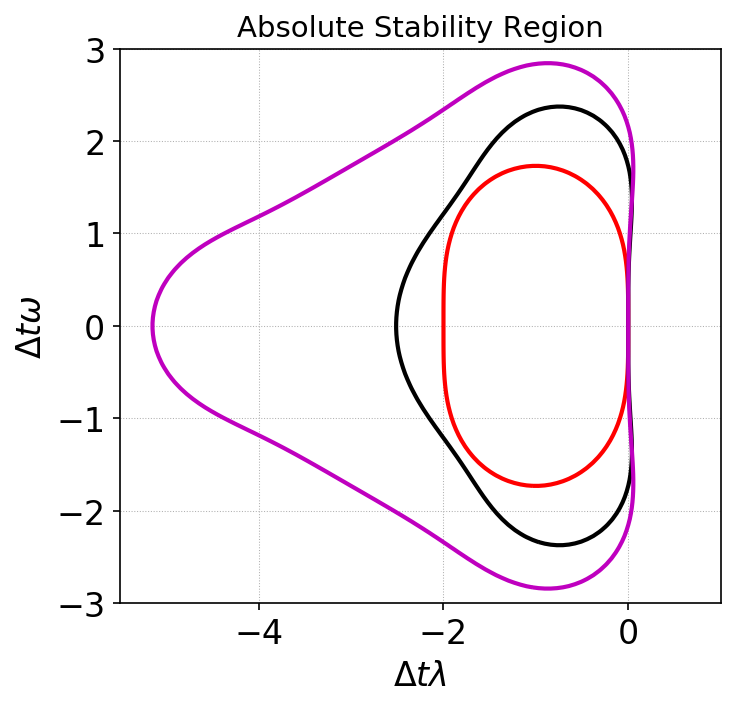
\includegraphics[width=\linewidth]{ssp-rk-abs-stability.png}
    \end{column}
  \end{columns}  
  
\end{frame}

\begin{frame}{Time-scales in a physical system}
  In typical plasmas the space and time-scales are enormous: plasma-
  and electron cyclotron-frequencies; light waves; sound waves, Alfven
  waves; (all MHD waves); resistive relaxation; transport scales. It's
  an orgy of scales! How to handle all these scales?
  \begin{itemize}
  \item One option: order out scales you do not care about by deriving
    asymptotic equations. Great example: extended MHD; gyrokinetics.
  \item However, these equations are still multi-scale! Worse, often
    there is no clean scale-separation in many interesting problems.
  \end{itemize}
\end{frame}

\begin{frame}{Time-scales in a model problem}
  \begin{columns}
    
    \begin{column}{0.5\linewidth}
      \small%
      Consider advection-diffusion-reaction-oscillation equation
      \begin{align*}
        \pfrac{f}{t} + a\pfrac{f}{x} = \nu \frac{\partial^2 f}{\partial x^2} + i\Omega f - \gamma f
      \end{align*}
      Here $\gamma \ge 0$ and $\Omega$ are real. Consider a single mode
      in space-time $e^{-i\omega t}e^{i k x}$ and get dispersion relation
      \begin{align*}
        \omega = \underbrace{(a k - \Omega)}_{ \omega}
        - i \underbrace{(\nu k^2 + \gamma)}_{-\lambda}
      \end{align*}
      For stability of explicit scheme we must choose
      $\omega \Delta t$ to lie inside the stability region of the
      time-stepping scheme.
    \end{column}
    
    \begin{column}{0.4\linewidth}
      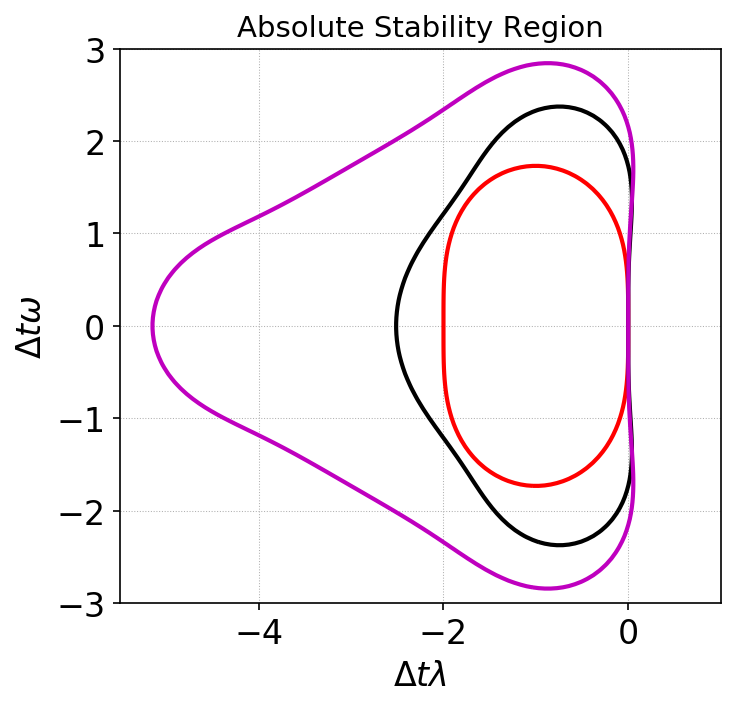
\includegraphics[width=\linewidth]{ssp-rk-abs-stability.png}
    \end{column}
  \end{columns}

\end{frame}

\begin{frame}{Time-scales in a model problem}
  For finite-difference schemes $k_{\textrm{max}} = 2/\Delta x$. Hence
  we have
  \begin{align*}
    \omega = \left(\frac{2a}{\Delta x}  - \Omega\right) -
    i \left(\frac{4\nu}{\Delta x^2} + \gamma \right)
  \end{align*}
  Depending on the regime one or the other term may dominate. For
  example, $\Omega$ may be very large.  Also, in particular, note that
  the damping from diffusion goes as $1/\Delta x^2$. This can be a
  serious limitation for explicit schemes.
  \begin{itemize}
  \item To overcome time-step limitation from $\Omega$ (oscillations)
    we need to use some sort of \emph{time-centered implicit method};
    For stiff $\gamma >> 1$ we need an damped implicit scheme.%
    \mypause%
  \item For diffusion dominated problems we can use implicit methods,
    or, preferably \emph{super time-stepping schemes} (STS schemes).%
    \mypause%
  \item For advection dominated problems explicit schemes are
    best. Implicit schemes for \emph{hyperbolic} equations are hard
    and do not always work well.
  \end{itemize}
\end{frame}

\begin{frame}{``Super-Time Stepping'' Schemes}
  \begin{columns}
  
    \begin{column}{0.5\linewidth}
      \begin{itemize}
      \item ``Super-Time Stepping'' or Runge-Kutta-Legendre (or
        Runge-Kutta-Chebyshev or ROCK2) schemes work by taking large
        (10-100s) of RK stages to increase region of stability along
        negative real axis.%
        \mypause%
      \item For $s$ stages the stability increases as $s^2$: hence,
        for large $s$ we can get an approximate $s\times$ speed up
        compared to explicit scheme.%
        \mypause%
      \item Note that STS schemes \emph{look} like explicit schemes!
        No need for complicated linear/nonlinear solvers.
      \end{itemize}
    \end{column}
    
    \begin{column}{0.5\linewidth}
      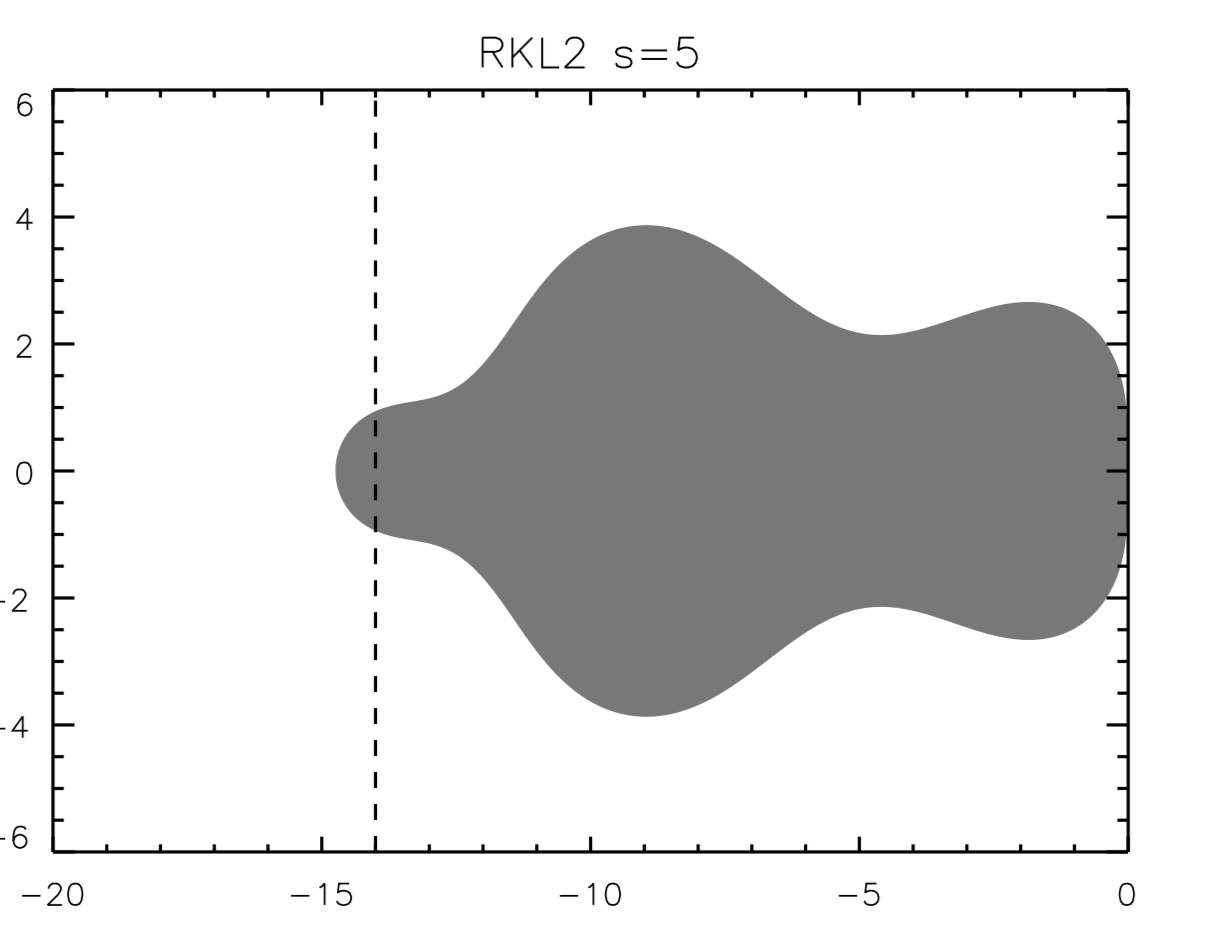
\includegraphics[width=\linewidth]{STS-RKL-5.png}
    \end{column}

  \end{columns}
\end{frame}

\begin{frame}{Time-stepping a complex system of equations}
  To summarize: to update a complex system of nonlinear equations with
  hyperbolic, parabolic, oscillating and reaction terms:
  \begin{itemize}
  \item For advection terms typically use explicit schemes: implicit
    schemes are hard. Limited by fastest eigenvalue in the system.
  \item For oscillating terms use a time-centered implicit scheme (or
    backward implicit for fastest oscillations); for reactions use a
    backward implicit scheme;
  \item For diffusion (even nonlinear diffusion) use a STS scheme.
  \end{itemize}
  In a real problem all these need to be combined using \emph{operator
    splitting} approaches.
\end{frame}

\end{document}


\begin{frame}{}
\end{frame}

\begin{columns}
  
  \begin{column}{0.6\linewidth}
  \end{column}
  
  \begin{column}{0.4\linewidth}
    \includegraphics[width=\linewidth]{fig/Kinsey_2011_Pfus_vs_T.pdf}
  \end{column}
\end{columns}

% ----------------------------------------------------------------
